%; whizzy chapter
% -initex iniptex -latex platex -format platex -bibtex jbibtex -fmt fmt
% 以上 whizzytex を使用する場合の設定。


%     Tokyo Debian Meeting resources
%     Copyright (C) 2007 Junichi Uekawa

%     This program is free software; you can redistribute it and/or modify
%     it under the terms of the GNU General Public License as published by
%     the Free Software Foundation; either version 2 of the License, or
%     (at your option) any later version.

%     This program is distributed in the hope that it will be useful,
%     but WITHOUT ANY WARRANTY; without even the implied warranty of
%     MERCHANTABILITY or FITNESS FOR A PARTICULAR PURPOSE.  See the
%     GNU General Public License for more details.

%     You should have received a copy of the GNU General Public License
%     along with this program; if not, write to the Free Software
%     Foundation, Inc., 51 Franklin St, Fifth Floor, Boston, MA  02110-1301 USA

%  preview (shell-command (concat "xpdf " (replace-regexp-in-string "tex$" "pdf"(buffer-file-name)) "&"))
% 画像ファイルを処理するためにはebbを利用してboundingboxを作成。
%(shell-command "cd image200701; ebb *.png")

%%ここからヘッダ開始。

\documentclass[mingoth,a4paper,twoside]{jsarticle}
\usepackage[dvipdfmx]{graphicx}
\usepackage{fancybox}
\usepackage{longtable}
\usepackage{ascmac}	% 囲み (screen,itembox)
\usepackage{fancyvrb}   % 囲み Verbatim のために必要
\usepackage[dvipdfmx]{hyperref}
\usepackage{url}
\usepackage[dvipdfmx]{color}
\usepackage{nextpage}
\usepackage{wrapfig}

% 日付を定義する、毎月変わります。
\newcommand{\debmtgyear}{2007}
\newcommand{\debmtgdate}{20}
\newcommand{\debmtgmonth}{1}
\newcommand{\debmtgnumber}{24}



%http://www.naney.org/diki/dk/hyperref.html
%日本語EUC系環境の時
\AtBeginDvi{\special{pdf:tounicode EUC-UCS2}}
%シフトJIS系環境の時
%\AtBeginDvi{\special{pdf:tounicode 90ms-RKSJ-UCS2}}

%% spacing の設定をする。外枠を減らす。
\setlength\headheight{0mm}
\setlength\topmargin{-20mm}
\setlength\headsep{0mm}
\setlength\topskip{3mm}
\setlength\maxdepth{4pt}
\setlength\columnsep{6mm}
\setlength\textheight{252mm}
\setlength\topmargin{-5mm}
\setlength\textwidth{170mm}
\setlength\oddsidemargin{-5mm}
\setlength\evensidemargin{-5mm}

% commandline環境を定義。画面入出力についてはcommandline環境
% で表記する
\newenvironment{commandline}%
{\VerbatimEnvironment
  \begin{Sbox}\begin{minipage}{15cm}\begin{fontsize}{7.3}{7.3} \begin{BVerbatim}}%
{\end{BVerbatim}\end{fontsize}\end{minipage}\end{Sbox}
  \setlength{\fboxsep}{8pt}\fbox{\TheSbox}}


%%% start of santaku
\makeatletter
\newwrite\tf@jqz
\immediate\openout\tf@jqz\jobname.jqz\relax
\makeatother
\newcounter{santakucounter}
\newcommand{\santaku}[5]{%
\addtocounter{santakucounter}{1}

\addtocontents{jqz}{\arabic{santakucounter}. #5\\}
\begin{minipage}{1\hsize}
問題\arabic{santakucounter}. 
#1\\
□ A #2\\
□ B #3\\
□ C #4
\end{minipage}
\hspace{1cm}
\\

}
%%% end of santaku

\newcommand{\emptyspace}{(\underline{\hspace{1cm}})}

\newcommand{\subsubsubsection}[1]{%
\vspace{1zw}{\bf #1}\\}


% sectionをセンタリングする
\makeatletter
  \renewcommand{\section}{\@startsection{section}{1}{\z@}%
    {\Cvs \@plus.5\Cdp \@minus.2\Cdp}% 前アキ
    {.5\Cvs \@plus.3\Cdp}% 後アキ
    {\normalfont\gt\fontsize{32}{32}\headfont\raggedright}} % style
\makeatother

% section の代わりの環境
\newcommand{\dancersection}[2]{%
\newpage
第\debmtgnumber{}回 東京エリアDebian勉強会 \debmtgyear{}年\debmtgmonth{}月
\hrule
\vspace{0.5mm}
\hrule
%
\vspace{4cm}
\hrule
\vspace{0.5mm}
\hrule
%
\vspace{-7cm}
\begin{minipage}[b]{0.7\hsize}
\section{#1}
\hfill{}#2\\
\vspace{2cm}
\end{minipage}
\begin{minipage}[b]{0.3\hsize}
\hfill{}
\includegraphics[height=8cm]{image200502/openlogo-nd.eps}\\
\end{minipage}
%
%\hfill{}
\includegraphics[width=16cm]{image2006-natsu/guruguru-sand-light.png}\\
\vspace{-1cm}
}

% BTSの番号を見るためのコマンド
\newcommand{\debianbug}[1]{Bug\##1\footnote{\url{http://bugs.debian.org/#1}}}

% for dancerj
\newcommand{\fgref}[1]{図\ref{#1}}
\newcommand{\tbref}[1]{表\ref{#1}}




\begin{document}

\begin{titlepage}

% 毎月変更する部分, 本文の末尾も修正することをわすれずに


 第\debmtgnumber{}回 東京エリア Debian 勉強会資料

\vspace{2cm}

\begin{minipage}[t]{0.6\hsize}
\vspace{-2cm}
{\fontsize{60}{60}
{\gt
東京エリア \\
デビアン \\
勉強会
}}
\end{minipage}
\begin{minipage}[b]{0.4\hsize}
\hspace{-1cm}
\includegraphics[width=9cm]{image200502/openlogo-nd.eps}
\end{minipage}

\vspace{3cm}
\hfill{}Debian勉強会幹事 上川 純一\\
\hfill{}\debmtgyear{}年\debmtgmonth{}月\debmtgdate{}日

\thispagestyle{empty}
\end{titlepage}

\dancersection{Introduction}{上川 純一}
 
 今月のDebian勉強会へようこそ。
 これからDebianのあやしい世界に入るという方も、すでにどっぷりとつかってい
 るという方も、月に一回Debianについて語りませんか?

 目的として次の二つを考えています。

 \begin{itemize}
 \item メールではよみとれない、もしくはよみとってられないような情報につ
       いて情報共有する場をつくる
 \item Debianを利用する際の情報をまとめて、ある程度の塊として整理するた
       めの場をつくる
 \end{itemize}

 Debianの勉強会ということで究極的には参加者全員がDebian Packageをがりがり
 と作るスーパーハッカーになった姿を妄想しています。

 Debianをこれからどうするという能動的な展開への土台としての空間を提供し、
 情報の共有をしたい、というのが目的です。


\newpage

\begin{minipage}[b]{0.2\hsize}
 \definecolor{titleback}{gray}{0.9}
 \colorbox{titleback}{\rotatebox{90}{\fontsize{80}{80} {\gt デビアン勉強会} }}
\end{minipage}
\begin{minipage}[b]{0.8\hsize}
\hrule
\vspace{2mm}
\hrule
\tableofcontents
\vspace{2mm}
\hrule
\end{minipage}

\dancersection{事前課題}{上川 純一}

今回の事前課題は
「今後、勉強会につかう施設を提案してください」と「2007年の勉強会の各月のアジェンダを提案してください」
というタイトルで200-800文字程度の文章を書いてください。というものでした。
その課題に対して下記の内容を提出いただきました。

\subsection{Ishihara さん}

\subsubsection{「今後、勉強会につかう施設を提案してください」}

角筈地域センター
\url{http://www2.odn.ne.jp/~hak35040/index.html}
公共の施設が安くて便利そうな気がします。
ただ、電源やLANとかそういう設備が厳しいのかもしれません。
個人的にはこういうところでの勉強会もやってみたいかも。
\url{http://www.tef.or.jp/oshima/index.html}

\subsubsection{「2007年の勉強会の各月のアジェンダを提案してください」}

・古いPC復活大作戦
\begin{enumerate}
 \item 古いマシンをDebianで復活させる:    古いマシン独特の問題
 \item デスクトップ機にしてみる:  Xつかうよ or Xつかわないよ
 \item サーバにしてみる:      セキュリティの問題
\end{enumerate}
みたいな感じで、ちょっと型落ちなマシンを復活させる、という実践的?な企画が
あってもいいかなぁと思います。
1年でサーバマシンが立てられるよ、セキュリティもちゃんと配慮できるよ、みたいな企画ですね。

あとは、Debianに関係する英語を読んで見ましょう企画とか。

・vs 英語
\begin{enumerate}
 \item Debianの英語サイトを読んでみよう:
     キーワードの見つけ方、
     英語の辞書の使い方、
     どのドキュメントを読めばいいの?
\end{enumerate}
やっぱりネックとなるのは英語なメッセージやドキュメントだと思います。
ググれ、と突き放すのもひとつの勉強法なんですけど、
ちょっとでも読み方がわかると、敷居が低くなるんじゃないのかなぁと思うのですが。
どうなんでしょうか?

\subsection{小林儀匡}

\subsubsection{『今後、勉強会につかう施設を提案してください』}
これまで何回か「大学は利用できないのか」という話があったこともあり、
大学所属のメンバーとして、勉強会に使える施設が大学内にないか検討してみました。

まず、情報教育のための施設である情報教育棟
\footnote{\url{http://www.edu.c.u-tokyo.ac.jp/}}については、『情報教育棟 
会議室・セミナー室利用申込』
\footnote{\url{http://www.edu.c.u-tokyo.ac.jp/etc/application.htm}}の利
用規定第2条(1)に、教職員が学部、専攻(系)、学科、部会、センター、委員会、
事務部が主宰する会合、とありました。
学生がサークルのようなものの集まりとして使用するような使い方はできないようです。
まぁ、
得体の知れない人間にコンピュータやネットワークを自由に利用されても困りますので、
仕方がないでしょうか。

次に、
サークルなどで使われている東京大学駒場コミュニケーション・プラザ\footnote{\url{http://www.com-pla.com/}}も検討してみました。
こちらの利用規則\footnote{\url{http://www.com-pla.com/kitakan/riyo.html}}には次のようにあります。

(中略)

例外的に適当と認められるために何をすればよいのかよくわかりませんが、
それなりの手続きを経なければいけないようです。

大学という場はオープンで結構使いやすいかと思われがちですが、
オープンすぎて勝手に使われると問題になるので案外色々と制限 (「主催者が教職員」とか「構成員が学内の人間」とか) がかかっていることが多いです。
昨年11月の大阪電気通信大学での勉強会のように教員が誘致してくださったりする場合はやりやすいでしょうが、
そうでない場合はなかなか使いにくい場ではないでしょうか。
まだまだ探す余地はあると思うのでもう少し粘ろうかと思いますが……。

\subsubsection{『2007年の勉強会の各月のアジェンダを提案してください』}

{\small
\begin{description}
 \item[2月] 「今年、私はDebianにこのように関わろうと思います/○○を成し遂げます!!」宣言大会
 \item[3月] Debian etchリリース記念インストール大会
 \item[4月] Debian lennyに向けて日本語圏でやっておきたい事項のリストアップ
 \item[5月] Debianを使っていて思う「このようなフリーなアプリケーションが足りない」
 \item[6月] Debian Conference 7現地報告
 \item[7月] Debian Conference 7報告
 \item[8月] Debianでのウェブアプリケーションのあれこれ
 \item[9月] Debianでのグラフィックアプリケーションのあれこれ
 \item[10月] Debianの派生ディストリビューションのあれこれ
 \item[11月] Debianと私
 \item[12月] 「今年、私はDebianに関して○○を成し遂げました/成し遂げられませんでした」報告・反省大会
\end{description}
}

\subsection{前田 耕平さん}

\subsubsection{「今後、勉強会につかう施設を提案してください」}

二箇所提案します。

\begin{enumerate}
 \item  晴海区民館:
 晴海トリトンにあります。ちょっと高いのが難点です。
 \url{http://www.city.chuo.lg.jp/sisetugaido/syukaisisetu/syukaisisetu17/}

 \item 月島区民館
 宴会を月島のお好み焼きや、もんじゃ焼きに絞る場合はこちらの方が良いかも。
	(ただ、月島の店は閉店が早いです。23時にしまっちゃいます)
	\url{http://www.city.chuo.lg.jp/sisetugaido/syukaisisetu/syukaisisetu14/index.html}
\end{enumerate}

あまり現実的ではありませんが、私の住んでいるマンションの共有施設、という手もあります。
利用料は安いのですが(300円or500円/1時間)、交通の便があまりよくありません。
あと、近くに飲み屋どころか、飲食店がほとんどありません。(あっても23時で閉店なので)
だからといってウチで飲み会、というのは困るので…。


\subsubsection{「2007年の勉強会の各月のアジェンダを提案してください」}

バッティングしそうなのもあるので、ネタだけ列挙します。

{\small
\begin{enumerate}
 \item Debianでだってできる3Dデスクトップs 裏番組(Vista)をぶっ潰せ!
 \item Etchリリース(仮)を祝って、Sarge→Etchのアップグレード苦労話
 \item 新入生・新入社員をDebianユーザにする企て
 \item 打ち上げ花火でDebianのグルグルを実現できるか(趣旨違いますね)
 \item Debian勉強会@Linux World又はLC(って今年も開催するのか?)
 \item 他のユーザ会とのコラボ(特にターゲットは無し)
\end{enumerate}
}

\subsection{岩松 信洋}


\subsubsection{ 「今後、勉強会につかう施設を提案してください」}

自分の勤務地の最寄り駅である国分寺駅近辺の施設を調べてみました。
いいところがありませんでした。
	
	
\subsubsection{「2007年の勉強会の各月のアジェンダを提案してください」}
{\small
\begin{itemize}
 \item	 2月 パッケージ依存関係を図にして印刷してみる:
		apt-cache dotty で出力された dotty ファイルをプリントアウト
		して満足する。
		
 \item	 3月 東京青少年オリンピックセンター 合宿 and OSC 2007 spring:
		合宿をする。
		OSC に参加して本を売る。

 \item	 4月 dbs を調べてみる:
		あまりメジャーではない dbs について熱く語る。

 \item	 5月 defoma を解析して、熱く語る。:
		山根さんが defoma を解析して、熱く語る。

 \item	 6月 debconf and OSC DO 2007:
		debconf組がエジンバラに行っている間、残った人はみんな
		北海道で合宿。

 \item	 7月 apt-xxx を調べる:
		実はみんなが知らない apt-xxx があるのではないか?
		調べて熱く語る。

 \item	 8月  ラインセンスを調べる  and コミケ:
		Debian パッケージの ライセンスを全て調べてみる。
		コミケをがんばる。

 \item	 9月 OSC 2007 Tokyo Fall に参加:
		OSCに参加する。

 \item	 10月 Debian で 動画再生環境を作ってみる:
		main セクションだけで動画再生環境を作ったらどうなるか、調べる。

 \item 	 11月 KOF に参加:
		KOFに参加して、○○\footnote{編集注:不適切
な表現があったため、削除)}さん実家に泊まる。

 \item	 12月 反省会 and コミケ:
		コミケをがんばる。
		反省会もちゃんとする。
		温泉合宿を決行する。
\end{itemize}
}

\subsection{北原さん}


\subsubsection{今後、勉強会につかう施設を提案してください}

  現在と同じような勉強会(曜日・時間・人数・プロ
ジェクター等の施設)が出来る施設を探してみました。
現在利用している施設の使用料がわからないので、参加
費と人数、資料代等を適当に勘案して、1万円以下を条
件としました。

  そうすると、民間の物件はほとんど不可能なので、
公共の施設となりますが、区の施設では利用者の制限が
厳しい(半数が区民である必要がある等)ので都の施設
を調べてみました。

  以前の勉強会で話題に挙がった、東京体育館、同じ
団体で管理している東京武道館・駒沢オリンピック公園
総合運動場・東京辰己国際水泳場(全て会議室あり)を
除くとあまり良いのは見つかりませんでした。

  その中でも「東京スポーツ文化館・BumB」が、利用
条件が緩く、2,625円からで利用できそうです(場所は夢の
島)。 勉強会に「男女平等の推進に関する」テーマが
盛り込めれば、「東京ウィメンズプラザ」(場所は神宮
前)が利用できるかも?(笑)(3,300円から)

  夜でなくても良ければ「東京国際ユースホステル」
の研修室が利用でるかも?(飯田橋の駅側、3,000円)

  あと、利用方法が調べきれていませんが、清澄庭園
・蘆花恒春園でも集会所が借りられるようですが、ちょ
いと勉強会とは雰囲気が違うような気がする。

  国関係も調べようと試みましたが、まったく引っか
かりませんでした。(調べ方が悪かったかも)

  あと、「東京スポーツ文化館・BumB」は宿泊施設が
あって最大251人(定員)泊まれます。 DebConfの検討
対象にはなりませんかね?



\subsection{小室 文さん}

\subsubsection{今後、勉強会につかう施設を提案してください}

練馬区在住なので、練馬区施設関連を中心に探しました。

貫井地区区民館\footnote{\url{http://www.city.nerima.tokyo.jp/chiiki/chikukan/kakukan/nukui.html}}
最寄:中村橋駅(西武池袋線)徒歩5分
1時間400円

光が丘地区区民館
\footnote{\url{http://www.city.nerima.tokyo.jp/chiiki/chikukan/kakukan/hikari.html}}
最寄:光が丘駅(大江戸線)
1時間:500円

石神井公園区民交流センター
\footnote{\url{http://www.city.nerima.tokyo.jp/kouryu/}}
最寄:石神井公園(西武池袋線)
会議室(1):1200円

練馬女性センター
\footnote{\url{http://www.city.nerima.tokyo.jp/jinken/indexj.html}}
最寄:石神井公園駅(西武池袋線)
第1研修室:1400円

後は学校開放というのをしていて、会議室がある小学校が夜間貸し出しをしてい
る所があるようです。
\footnote{\url{http://www.city.nerima.tokyo.jp/nerima_sg/manabi/kaihou.html}}
夜間は18時から21時で、大体600円ぐらいです。

練馬まで来てくれるかっというのが最大の問題ですね・・・

\subsubsection{2007年の勉強会の各月のagenda}

暗号化とは!?とか・・自分で調べたら分かるよなぁという事もただあるので、
なかなか思いつかないですね。「これだけは絶対やってはいけない操作」とかど
うでしょう。後は個人的にDebian policyは勉強したいと思います。ちゃんとし
た回答になっていなくてすいません・・・



%%% trivia quiz
\dancersection{Debian Weekly News trivia quiz}{上川 純一}

ところで、Debian Weekly News (DWN)は読んでいますか?
Debian 界隈でおきていることについて書いているDebian Weekly News.
毎回読んでいるといろいろと分かって来ますが、一人で読んでいても、解説が少
ないので、
意味がわからないところもあるかも知れません。みんなでDWNを読んでみましょう。

漫然と読むだけではおもしろくないので、DWNの記事から出題した以下の質問にこたえてみてください。
後で内容は解説します。

\subsection{2006年42号}
\url{http://www.debian.org/News/weekly/2006/42/}
にある2006年12月26日版です。

\santaku
{Linux Conference Australia で開催される Debian 関係のイベントは今回で何回目か}
{1}
{3}
{6}
{C}

\santaku
{最近急上昇してDebian内で3位人気のアーキテクチャになったアーキテクチャは?}
{ARM}
{PPC}
{AMD64}
{A}

\santaku
{etchがフリーズされたのはいつ?}
{11/11}
{12/11}
{12/24}
{B}

\santaku
{Debian のインストール CD イメージはどれくらいの頻度で更新されているか?}
{毎日}
{毎メジャーリリース}
{毎マイナーリリース}
{A}
\dancersection{最近のDebian関連のミーティング報告}{上川 純一}

\subsection{東京エリアDebian勉強会23回目報告}
% (query-replace-regexp "<.*>" "")


   	  東京エリアDebian勉強会報告。
	  12月の第23回Debian勉強会を実施しました。
	    Bug Squashing Party について報告するのと、一年間のDebian 勉強会を反省する会です。
	  
	  今回の参加人数は15人でした。
	  あけどさん、小室さん、小林さん、岩松さん、Henrichさん、前田さん、澤田さん、キタハラさん、青木さん、みつかさん、えとーさん、
	  でんさん、野首さん、gotomさん、上川でした。
        
	
	  
	    まず、事前課題の紹介をしました。来年のスタイルについてのみ
	    なさまの提案をいただきました。今Debianの各種インタフェース
	    がどうなっているのかドキュメントを作成している、それには価
	    値がある、という話や、会場で実習する「ハンズオン」ができる
	    と、忘れないうちに体験できるのでよいよね、という話題、ネッ
	    トワークの事前課題で出てきたような特定のトピックにまつわる
	    バッドノウハウをたくさん集めるというのを今後もやりたいとい
	    うのが出てきました。また、用語がわからないというかまったく
	    ついていけない場合があるのだが、そういうのをログをとってお
	    いて後から質問できるようになっているとよいのではないかとい
	    う提案などがありました。
	  
	  
	    岩松さんと gotom さんが、先日開催した Bug Squashing Party 
	    についての報告を実施しました。今回のBSPでは、etchリリース
	    直前ということもあり、難しいバグしか残っていないことで、日
	    本のメンテナのバグを修正するという方向を出してみました、と
	    のことです。BSP をやるまえに課題を洗い出してくださいという
	    メールを出すのはよいのではないかという提案がありました。今
	    後も開催したいのでBSP ができる会場を探したいそうです。まだ
	    よい会場をみつけれていないのですが、例えば二ヶ月に一回くら
	    い開催するために場所を探しているというメールを出したら誰か
	    良い場所を教えてくれるのではないか、というのが希望的観測で
	    した。
	  
	  
	    上川が今年一年のアクティビティーの結果をまとめて報告しまし
	    た。ふりかえってみるといろいろとみえてきます。今年は結果と
	    して7回は通常運用の方法で開催していましたが、6回は場所を外
	    部にとって違う場所で開催しているということが判明しました。
	    来年も半々くらいでやっていくのがよいんじゃないかと思います。
	    1月に実施内容を決定するようにしましょう、という話になりました。
	  
	  
	    宴会は荻窪 うさぎにて。素敵なお店でした。


\subsection{Debian Conference参加案内}

Debian Conference7 が開催されます。参加者は1月末日までに登録してください。

\begin{tabular}[t]{|r|l|}
\hline
場所 & イギリス エジンバラ \\
\hline
日時 & 2007年6月17日-23日\\
\hline
 ウェブページ & \url{http://debconf7.debconf.org}\\
\hline
\end{tabular}



\dancersection{apt-torrent}{岩松 信洋}
\label{sec:apt-torrnet}

Debian パッケージのレポジトリを \texttt{bittorrent} ネットワーク上に置き、それを apt で取得するというものが \texttt{apt-torrent} です。

まだ Debian としては頒布されておらず、フランス人の方が一人でシコシコやっているようです。\url{http://sianka.free.fr/} で開発が行われています。

\subsection{bittorrent とは}
bittorrent とは、P2P を用いたファイル転送用プロトコルとその通信を行うソフトウェアの事を指します。
特徴としては、P2P でファイルの一部をお互いに送受信しあうというプロトコルになっているところです。

通常の P2P ソフトウェアではファイルを提供元に集まるようになっているが、このプロトコルを使うこと
により、ネットワーク帯域のないピアもファイルの配布に協力できるようになっています。

このプロトコル上で Debian パッケージを頒布し、aptで取得するようにしたものが\texttt{apt-torrent}です。

\subsection{使い方}

\subsubsection{ダウンロード}
先にも書いたように Debian としては頒布されていません。

以下のサイトからダウンロードし、使用します。

\url{http://sianka.free.fr/download/apt-torrent_0.5.0-1_all.deb}

apt のソースとして利用できる apt-line も提供されており、以下の apt-line
を\texttt{/etc/apt/sources.list}に追記して使用可能です。
\begin{itemize}
	\item \url{deb http://sianka.free.fr/apt-torrent testing main}
	\item \url{deb-src http://sianka.free.fr/apt-torrent testing main}
	\item \url{deb http://sianka.free.fr/apt-torrent unstable main}
	\item \url{deb-src http://sianka.free.fr/apt-torrent unstable main}
\end{itemize}

\subsubsection{設定}
パッケージをインストールすると、自動的に \texttt{/etc/apt/sources.list} に追記されます。

以下が追加された \texttt{apt-torrent} 用の apt-line です。

\begin{commandline}
### BEGIN APT-TORRENT SOURCE LIST
# Do not edit or remove the markers, they are used by the apt-torrent package

# Uncomment one of the following:
# deb http://127.0.0.1:6968/debian/ unstable main
# deb http://127.0.0.1:6968/debian/ testing main

### END APT-TORRENT SOURCE LIST
\end{commandline}

自分の環境に合わせて apt-line のコメントを外します。

\subsubsection{apt-get update してみる}
apt-torrent 用の apt-line だけ有効にし、apt-get update を実行してみます。

\begin{commandline}
iwamatsu@chimagu:~$ LANG=C sudo apt-get update
Get:1 http://127.0.0.1 unstable Release.gpg [189B]
Get:2 http://127.0.0.1 unstable Release [776B]
Ign http://127.0.0.1 unstable/main Packages/DiffIndex
Get:3 http://127.0.0.1 unstable/main Packages [27.9kB]
Fetched 28.9kB in 3s (8118B/s)
Reading package lists... Done
\end{commandline} 

\subsubsection{ 何かパッケージをインストールしてみる }
いつも使っているapt-get / aptutide / dselect で torrent ネットワークから Debian Package を取得することが可能です。

しかし、実はどのようなパッケージが torrent 上にあるのか分りません。
ドキュメントを読む限り先の URI のサイトで公開されている apt 用のレポジトリ \url{deb http://sianka.free.fr/debian unstable main} にあるものが公開されているようです。

apt のフロントエンドである aptitude を使い、インストールしたときの例を以下に示します。

\begin{commandline}
# aptitude install frozen-bubble
Reading Package Lists... Done
Building Dependency Tree
Reading extended state information
Initializing package states... Done
Reading task descriptions... Done
The following NEW packages will be automatically installed:
 fb-music-high frozen-bubble-data
The following packages have been kept back:
 galeon galeon-common
The following NEW packages will be installed:
 fb-music-high frozen-bubble frozen-bubble-data
0 packages upgraded, 3 newly installed, 0 to remove and 2 not upgraded.
Need to get 12.1MB/12.2MB of archives. After unpacking 17.3MB will be used.
Do you want to continue? [Y/n/?]
Writing extended state information... Done
Get:1 http://127.0.0.1 unstable/main fb-music-high 0.1.1 [6950kB]
Get:2 http://127.0.0.1 unstable/main frozen-bubble-data 1.0.0-6 [5155kB]
Fetched 12.1MB in 24s (488kB/s)
Selecting previously deselected package fb-music-high.
(Reading database ... 208931 files and directories currently installed.)
Unpacking fb-music-high (from .../fb-music-high_0.1.1_all.deb) ...
Selecting previously deselected package frozen-bubble-data.
Unpacking frozen-bubble-data (from .../frozen-bubble-data_1.0.0-6_all.deb) ...
Selecting previously deselected package frozen-bubble.
Unpacking frozen-bubble (from .../frozen-bubble_1.0.0-6_i386.deb) ...
Setting up fb-music-high (0.1.1) ...
Setting up frozen-bubble-data (1.0.0-6) ...
Setting up frozen-bubble (1.0.0-6) ...

Reading Package Lists... Done
Building Dependency Tree
Reading extended state information
Initializing package states... Done
Reading task descriptions... Done
\end{commandline}

2007/01/18 現在では正常にパッケージが取得できません。\footnote{作者に連絡取り中}

\subsection{仕組み}

\texttt{apt-torrent} は torrent ネットワーク用のデーモンと、パッケージを取得するデーモンの二種類があります。
プロセスを見ると、\texttt{apt-torrent} のプロセスがあることがわかります\footnote{btlaunchmany は複数の seed 管理用デーモン}。

\begin{commandline}
23404 ?        Ssl    0:00 /usr/bin/pike7.6 /usr/bin/apt-torrent
23411 ?        S      0:00 /usr/bin/pike7.6 /usr/bin/apt-torrent-httpd
23412 ?        S      0:00 /usr/bin/python /usr/bin/btlaunchmany /var/cache/apt-torrent --max_upload_rate -1 --parse_dir_interval 7
23644 pts/0    R+     0:00 ps ax
\end{commandline}

\texttt{apt-torrnet} は ファイルを取得するデーモン、\texttt{apt-torrent-httpd} はデータを管理する httpd server です。
これら2つのデーモンが通信を行い、 \texttt{bittorrent}網から Debian Package を取得します。

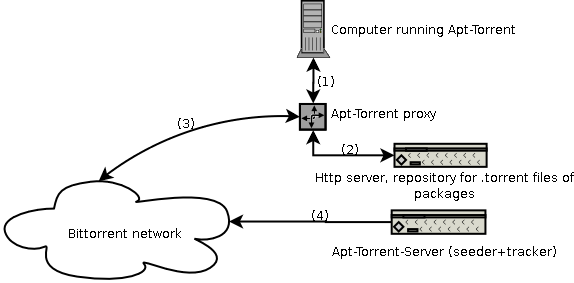
\includegraphics[width=15cm]{image200701/apt-torrent00.png}

簡単な流れは以下のようになります。
\begin{enumerate}
	\item クライアントで \texttt{apt-get update} を行います。

		行うと、\texttt{apt-torrent-proxy}を介して、通信を行います。

	\item \texttt{apt-torrent-proxy} を介して \texttt{apt-torrent} 用の http server と通信します。

		通信を行い、\texttt{/etc/apt/sources.list}に指定してある apt-line のサーバーから情報を取得を試みます。
	\item bittorrent 網 にアクセスします。
	
	\item \texttt{apt-torrent} server から一覧を取得します。

		\texttt{apt-torrent} は seeder\footnote{対象ファイルのデータを全て持っているピア} と 
		tracker\footnote{bittorrentファイルを管理するサーバー}を行っている \texttt{apt-torrent} にアクセスします。
	
	\item \texttt{apt-get install xxxxxxxx} を行います
		\texttt{apt-torrent-proxy} を介して、seeder からデータの取得を試みます。
		取得したデータは Debian Package なので aptが後は勝手に処理をします。
 	
\end{enumerate}

\texttt{apt-torrent} 用 http server を介して bittorrent 網にアクセスしているので、httpで公開されている apt-line から
パッケージを取得しているのと変わらない動きをします。

\subsection{apt との比較}
	今では、apt-get 時に http / ftpサーバーに負荷が集中していますが、\texttt{apt-torrent} を使用することによって
	ひとつのパッケージを ピア同士で共有することが可能になります。\texttt{apt-torrnet} は http / ftpサーバーに
	負荷がかからなくなるひとつの方法になるのではないかと個人的に考えています。
	変化が激しい unstable / testing は無理としても、stable のパッケージを \texttt{apt-torrent} で頒布するのはいい方法
	だと思います。今後、開発者と連絡を取り合い、自宅でも \texttt{apt-torrent} serverを立てて、実験してみようと模索し
	ているところです。
	
\subsection{その他}
 同じような機能を持った Winny のプロトコルを使い、\texttt{apt-winny}を実装してみると面白いと思いました。
 2ch で winny の Linux版である Linny を開発しているようなので(コードはまだない。)期待したいと思います。


\cleartoevenpage
\dancersection{Debian勉強会 2007年度計画}{上川 純一}
\label{sec:debmtg2007gw}

%偶数ページにきてほしい。

{\Large
Debianが今提供している付加価値は「\underline{\hspace{8cm}}」です。
2007年に発生しそうな外部的なイベントは次の項目です
\begin{itemize}
 \item Windows: (\underline{\hspace{8cm}})
 \item Mac OS X:(\underline{\hspace{8cm}})
 \item 他のディストリビューション: (\underline{\hspace{8cm}})
 \item ハードウェア: (\underline{\hspace{8cm}})
 \item ユーザの期待: (\underline{\hspace{8cm}})
 \item (\underline{\hspace{8cm}})
\end{itemize}

この状況を踏まえて Debian 勉強会が成し遂げるべきことは

「\underline{\hspace{8cm}}」です。

これらを踏まえて2007年のDebian 勉強会のテーマは

「\underline{\hspace{8cm}}」

とします。ここで、2007年の12ヶ月分のアジェンダを作成します。

\begin{enumerate}
 \item 新年会(\underline{\hspace{8cm}})
 \item (\underline{\hspace{8cm}})
 \item OSC? (\underline{\hspace{8cm}})
 \item OSC-Do? (\underline{\hspace{8cm}})
 \item Debconfプレゼンリハーサル (\underline{\hspace{8cm}})
 \item Debconfエジンバラ開催 (\underline{\hspace{8cm}})
 \item Debconf参加報告会(\underline{\hspace{8cm}})
 \item Debian 14周年 (\underline{\hspace{8cm}})
 \item (\underline{\hspace{8cm}})
 \item OSC-Fall? (\underline{\hspace{8cm}})
 \item KOF? (\underline{\hspace{8cm}})
 \item 忘年会(\underline{\hspace{8cm}})
\end{enumerate}

この中で自分が主体として開催するのは
「\underline{\hspace{8cm}}」の回の内容です。

名前のブランディングとして、
通常実施の勉強会を「\underline{\hspace{8cm}}」と呼び、
大衆向けの勉強会を「\underline{\hspace{8cm}}」と呼びます。

}

\dancersection{パッチ管理ツールquiltの使い方}{小林儀匡}
%\label{sec:quilt}

本節ではパッチ管理ツールquilt\footnote{\url{http://savannah.nongnu.org/projects/quilt}}を取り上げ、
その基本操作を中心に説明します。
quiltはDebianに特有な (つまりDebian-specificな) ソフトウェアではなく、
Debianとは全く関係のない場所で開発されています。
しかし、このツールがDebianパッケージの作成に有用であることを理解し、
実際に作成に使用してもらえたら嬉しい限りです。

\subsection{はじめに}

\subsubsection{パッチとは}

開発者であれば当然のように作成したり読んだり当てたりしたことがある\textbf{パッチ}ですが、
一般ユーザには見慣れないものだと思います。
そこで、最初にパッチについて説明しておきます。

パッチとは、2つのファイルの差分を含むファイルのことです。
次のような2つのファイルがあるとしましょう。

\begin{commandline}
nori1[3:57]%  cat file1.txt                                        saba:~/tmp/q
あいうえお
かきくけこ
さしすせそ
たちつてと
なにぬねの
はひふへほ
まみむめも
や ゆ よ
らりるれろ
わ を ん
nori1[3:58]%  cat file2.txt                                        saba:~/tmp/q
あいうえお
ばびぶべぼ
たちつてと
なにぬねの
まみむめも
や ゆ よ
らりるれろ
わ を ん
\end{commandline}

これらのファイルのどこが違っているかすぐにわかりますか?
一々目で比べる必要はありません。
\texttt{diff}コマンドでこれらの差分をとることができます。

\begin{commandline}
nori1[3:57]%  diff file1.txt file2.txt                             saba:~/tmp/q
2,3c2
< かきくけこ
< さしすせそ
---
> ばびぶべぼ
6d4
< はひふへほ
\end{commandline}

\texttt{file1.txt}と\texttt{file2.txt}の内容や行番号を考えれば、
なんとなく意味がわかると思います。
それでかまいません。
もちろん、この出力を手で書けるようにならなくてかまいません。

この形式でもよいのですが、
通常は\texttt{diff}コマンドに\texttt{-u}オプションをつけ、
次のような\textbf{unified diff}という形式で出力させます。

\begin{commandline}
nori1[3:57]%  diff -u file1.txt file2.txt                          saba:~/tmp/q
--- file1.txt   Thu Jan 18 03:57:14 2007
+++ file2.txt   Thu Jan 18 03:57:22 2007
@@ -1,9 +1,7 @@
 あいうえお
-かきくけこ
-さしすせそ
+ばびぶべぼ
 たちつてと
 なにぬねの
-はひふへほ
 まみむめも
 や ゆ よ
 らりるれろ
\end{commandline}

こちらのほうが、
追加・削除された行がどちらのファイルに所属するのか、
そしてファイルのどのような部分が異なるのかがわかりやすいでしょう。

パッチとは要は、次のようにしてこういった出力をファイルに収めたものです。

\begin{commandline}
nori1[3:58]%  diff -u file1.txt file2.txt > file.diff              saba:~/tmp/q
\end{commandline}

ただし、全く縁のない2つのファイルであれば差分はわざわざファイルに収める必要はないでしょう。
わざわざパッチを作成するのは、
ファイルに変更を加える前後の差分を見たり、
後で紹介するように機械的な処理で変更を加えられるようにしたりするためです。
そこで、
ここまでは\texttt{file1.txt}と\texttt{file2.txt}は無縁のファイルとしてきましたが、
ここからは\texttt{file1.txt}を改変したものが\texttt{file2.txt}であると考えてください。
つまり\texttt{file1.txt}が改変前のファイルで、
\texttt{file2.txt}が改変後のファイル、
パッチ\texttt{file.diff}には\texttt{file1.txt}を\texttt{file2.txt}にするための変更が含まれている、
と考えてください。

さて、作成したパッチは、\texttt{patch}コマンドを用いて、
その中に含む変更を該当ファイルに\textbf{適用する} (\textbf{当てる}) ことができます。

\begin{commandline}
nori1[4:00]%  patch < file.diff                                    saba:~/tmp/q
patching file file1.txt
\end{commandline}

こうして\texttt{file1.txt}の内容は\texttt{file2.txt}の内容と同一になります。

\begin{commandline}
nori1[4:01]%  cat file1.txt                                        saba:~/tmp/q
あいうえお
ばびぶべぼ
たちつてと
なにぬねの
まみむめも
や ゆ よ
らりるれろ
わ を ん
nori1[4:02]%  cmp file1.txt file2.txt                              saba:~/tmp/q
\end{commandline}

また、\texttt{-R}オプションを指定して逆向きに当てることもできます。

\begin{commandline}
nori1[4:18]%  patch -R < file.diff                                 saba:~/tmp/q
patching file file1.txt
nori1[4:19]%  cat file1.txt                                        saba:~/tmp/q
あいうえお
かきくけこ
さしすせそ
たちつてと
なにぬねの
はひふへほ
まみむめも
や ゆ よ
らりるれろ
わ を ん
\end{commandline}

\texttt{file1.txt}の内容は元に戻りました。

パッチは必ずしもうまく当たらないことを忘れてはなりません。
次のように、\texttt{file1.txt}の2行目を手元で改変したとします。

\begin{commandline}
nori1[5:29]%  cat file1.txt                                        saba:~/tmp/q
あいうえお
がぎぐげご
さしすせそ
たちつてと
なにぬねの
はひふへほ
まみむめも
や ゆ よ
らりるれろ
わ を ん
\end{commandline}

これに先程のパッチを当てようとすると次のようにエラーになります。

\begin{commandline}
nori1[5:30]%  patch < file.diff                                    saba:~/tmp/q
patching file file1.txt
Hunk #1 FAILED at 1.
1 out of 1 hunk FAILED -- saving rejects to file file1.txt.rej
\end{commandline}

これは、手元で与えた変更とパッチが加えたい変更が競合しているからです。

もちろん、\texttt{file1.txt}の2行目を改変する代わりに、
次のように最終行に1行加えたとします。

\begin{commandline}
nori1[5:32]%  cat file1.txt                                        saba:~/tmp/q
あいうえお
かきくけこ
さしすせそ
たちつてと
なにぬねの
はひふへほ
まみむめも
や ゆ よ
らりるれろ
わ を ん
むふふふふ
\end{commandline}

この場合、
手元で加えた変更はパッチが含む変更とは被らないので、パッチはうまく当たります\footnote{ただしあくまで形式的にであって、意味的に適切かどうかは確認する必要があります。}。

\begin{commandline}
nori1[5:36]%  patch < file.diff                                    saba:~/tmp/q
patching file file1.txt
nori1[5:52]%  cat file1.txt                                        saba:~/tmp/q
あいうえお
ばびぶべぼ
たちつてと
なにぬねの
まみむめも
や ゆ よ
らりるれろ
わ を ん
むふふふふ
\end{commandline}

これまでは1つのファイルの変更を1つのパッチに収めてきましたが、
1つのパッチに複数のファイルの変更を収めることも可能です。
以下は、\texttt{diff}に\texttt{-r}オプションを渡して、
内容の一部が異なる2つのファイルを含む2つのディレクトリの差分をパッチとして出力させた例です。

\begin{commandline}
nori1[5:14]%  diff -ur skkdic.orig skkdic > skkdic.diff              saba:~/tmp
nori1[5:14]%  cat skkdic.diff                                        saba:~/tmp
diff -ur skkdic.orig/debian/changelog skkdic/debian/changelog
--- skkdic.orig/debian/changelog        Fri Dec 15 03:36:49 2006
+++ skkdic/debian/changelog     Mon Dec 25 17:39:10 2006
@@ -1,5 +1,7 @@
 skkdic (20061130-2~pre1) unstable; urgency=low
 
+  * debian/rules: Pass the `-k' option to dh_installchangelogs so that
+    all of ChangeLog* are installed equally.
   * debian/skkdic{,-cdb,-extra}.docs: Deleted since their settings are
     now moved into debian/rules.
 
diff -ur skkdic.orig/debian/rules skkdic/debian/rules
--- skkdic.orig/debian/rules    Fri Dec 15 03:36:49 2006
+++ skkdic/debian/rules Mon Dec 25 17:39:10 2006
@@ -2,6 +2,7 @@
 include /usr/share/cdbs/1/rules/debhelper.mk
 include /usr/share/cdbs/1/class/makefile.mk
 
+DEB_DH_INSTALLCHANGELOGS_ARGS := -k
 DEB_INSTALL_CHANGELOGS_ALL := ChangeLog
 DEB_INSTALL_DOCS_ALL := ChangeLog.* READMEs/committers.txt
 
\end{commandline}

以上で簡単なパッチの説明は終わりです。
こういったパッチは、
修正した部分を確認したり他人と修正内容をやりとりしたりするのに非常に便利で、
開発作業はこれなしではやっていけないと言っても過言ではないでしょう。
実際に使うに当たってはpatch(1)やdiff(1)を参照することをお勧めします。

\subsubsection{パッチ管理ツールとは}

今回説明するquiltはパッチ管理ツールです。
これは、複数のパッチを管理するためのものです。
どのような場合に必要になるのでしょう?

先程パッチとは「修正した部分を確認したり他人と修正内容をやりとりしたりするのに非常に便利」だと書きました。
その言葉に基づけば、一般にはパッチとは使い捨ての一時ファイルで短寿命です。
管理する必要はありません。

しかし、以下のようなケースを考えてみてください。
\begin{itemize}
 \item ある団体がソフトウェアfooを公開し、定期的にリリースしている。
 \item Aさんはfooを改変して使ったり再配布したりする必要がある。
 \item Aさんの改変内容には複数の論理的に異なる変更が混ざっており、fooに取り込まれるものもあれば取り込まれないものもある。
\begin{itemize}
 \item fooのバグの修正1 (小さな変更なので次のマイナーリリースで適用される。)
 \item fooのバグの修正2 (大きめの変更なので次のメジャーリリースまで適用されない。)
 \item fooのバグの修正3 (バグを回避するためのAさん独自の次善策で、開発元からのリリースでは適用されない。)
 \item :
 \item fooのバグの修正N
 \item Aさんの環境に合わせるためのMakefileの修正
\end{itemize}
\end{itemize}

Aさんが全体の変更を1つのパッチとして管理するのは不可能に近いでしょう。
fooの新しいリリースが出たときに、
元のパッチを当てても (うまく当たる部分もあるでしょうが) 間違いなくうまく当たりません。
しかも複数の変更が混ざっているのでそれを解決するのは非常に大変でしょう。

変更を複数の論理的なパッチに分割すれば、少しは管理が楽になるでしょう。
1つずつパッチを当て、うまく当たるものと当たらないものを区別できます。
当たらないもののうち、
既に開発元で加えられた修正のパッチは削除し、
残すべきなのに他の変更の影響で部分的にうまく当たらないパッチはうまく当たるよう調整します。
それらの作業は面倒かもしれませんが、
1つのパッチとして管理するのに比べれば楽でしょう。
ただし、作業中に、
現在どのパッチが当たっていてどれが当たっていないかを一々覚えておかなければならないのが大変です。

そこで登場するのがパッチ管理ツールです。
パッチ管理ツールは、複数のパッチの取り扱いを楽にするためのツールです。
具体的には、どのパッチが当たっておりどれが当たっていないかを管理できます。
また、一度に複数のパッチを当てたり外したりできるので、
全ての (あるいはある一群の) パッチがうまく当たるかどうかを概観するのも楽にできます。
Aさんがやっているような作業にはうってつけのツールです。

さて、実はDebianパッケージのメンテナ (保守担当者) はこのAさんのような作業をする必要があります。
すなわち、
開発元のリリースに複数のパッチを独自に当て、それらを管理する必要があるのです。
というのも、
一般に開発元とDebianとではリリースサイクルや品質の基準が異なるからです。
管理すべきパッチは、ソフトウェアの規模が大きくなればなるほど増えるでしょう。
そこでDebianパッケージメンテナはパッチ管理ツールを使用することが推奨されています。

ここではquiltを使用したパッチ管理を紹介します。
Debianでよく使われるパッチ管理ツールには、dpatchというものもあります。
こちらはDebianパッケージメンテナンスに特化したツールですが、
機能的にはquiltとそんなに違いはありません。
興味がある方は、2005年7月勉強会\footnote{\url{http://www.netfort.gr.jp/~dancer/column/2005-debianmeeting.html.ja\#6th}}の資料を参照してください。

\subsection{インストール}

quiltは、Debianでは\texttt{quilt}パッケージに含まれており、
\texttt{apt-get}や\texttt{aptitude}で普通にインストールできます。

\subsection{quiltの基本操作}

\subsubsection{最初に知っておくべきこと}

quiltでは一般に、\texttt{quilt <コマンド>}という書式で様々なコマンドが利用できます。
利用可能なコマンドの一覧は次のようにして参照できます。

\begin{commandline}
nori1[13:19]%  quilt --help                                             whale:~
使い方: quilt [--trace[=verbose]] [--quiltrc=XX] command [-h] ...
       quilt --version
コマンド一覧:
        add       files   import   previous  setup
        annotate  fold    mail     push      snapshot
        applied   fork    new      refresh   top
        delete    graph   next     remove    unapplied
        diff      grep    patches  rename    upgrade
        edit      header  pop      series

全コマンド共通オプション:

--trace
        コマンドをbashのトレースモード(-x)で実行。内部デバッグ用。

--quiltrc file
        ~/.quiltrc (存在しない場合は代わりに /etc/quiltrc) 以外のコン
        フィギュレーションファイルを指定。内容の詳細については PDFのド
        キュメントを参照。

--version
        バージョン情報を出力して終了。
\end{commandline}

また各コマンドのヘルプメッセージは各コマンドに\texttt{-h}オプションを指定すれば表示できます。
以下の例では\texttt{quilt add}のヘルプメッセージを表示させています。

\begin{commandline}
nori1[13:45]%  quilt add -h                                             whale:~
Usage: quilt add [-P patch] {file} ...

Add one or more files to the topmost or named patch.  Files must be
added to the patch before being modified.  Files that are modified by
patches already applied on top of the specified patch cannot be added.

-P patch
        Patch to add files to.
\end{commandline}

\subsubsection{パッチスタック}

実際にquiltを使う前に、quiltのデータ構造を知っておきましょう。
quiltは、あるツリーに対する一連のパッチを一列に並べてスタックとして管理します。

あるソースツリーに、以下のような5つのパッチを順に加えたいとします。

\begin{enumerate}
 \item r1091-remove-trailing-garbage.diff
 \item r1092-implement-distclean.diff
 \item r1094-add-readme.diff
 \item fix-ftbfs-on-m68k.diff
 \item work-around-an-error-of-libtool.diff
\end{enumerate}

このとき、
これらのパッチは\textbf{patchesディレクトリ}に含まれていなければなりません。
そして、パッチの整列順序を収めた次のような内容の\textbf{seriesファイル}\footnote{dpatchにおける\texttt{00list}と同じ役割を果たします。}がパッチディレクトリに含まれている必要があります。

\begin{screen}
\begin{verbatim}
r1091-remove-trailing-garbage.diff
r1092-implement-distclean.diff
r1094-add-readme.diff
fix-ftbfs-on-m68k.diff
work-around-an-error-of-libtool.diff
\end{verbatim}
\end{screen}

つまりまとめると、
上に挙げた5つのパッチを順に加えるようなパッチセットのデータは次のようなものです。

\begin{commandline}
nori1[14:22]%  ls patches/*             whale:~/svnwc/deb/serf/trunk/serf-0.1.0
patches/fix-ftbfs-on-m68k.diff
patches/r1091-remove-trailing-garbage.diff
patches/r1092-implement-distclean.diff
patches/r1094-add-readme.diff
patches/series
patches/work-around-an-error-of-libtool.diff
nori1[14:22]%  cat patches/series       whale:~/svnwc/deb/serf/trunk/serf-0.1.0
r1091-remove-trailing-garbage.diff
r1092-implement-distclean.diff
r1094-add-readme.diff
fix-ftbfs-on-m68k.diff
work-around-an-error-of-libtool.diff
\end{commandline}

quiltのパッチデータはこれが全てです。

なおこのデータ構造は、
\ref{subsubsec:quilt-create-patch}で後述するパッチ作成作業時にquiltが自動的に作成してくれるので、
通常は手でいじる必要はありません。
次のセクションでは、
このようなpatchesディレクトリを既にもったツリーでパッチを当てたり外したりしてみましょう。

\subsubsection{パッチスタックの操作}

さて、ではquiltを使ってみます。
まずはスタック管理のための操作を眺めてみましょう。
スタック管理に必要な操作は、もちろんpushとpopです。

最初は何もパッチが当たっていないとします。
この状態で\texttt{quilt push}を実行すると、
1番目のパッチ、つまり\texttt{r1091-remove-trailing-garbage.diff}が当たります。
このパッチは\texttt{Makefile.in}に修正を加えるものです。

\begin{commandline}
nori1[14:30]%  quilt push               whale:~/svnwc/deb/serf/trunk/serf-0.1.0
Applying patch r1091-remove-trailing-garbage.diff
patching file Makefile.in

Now at patch r1091-remove-trailing-garbage.diff
\end{commandline}

きちんと当たったようですね。
\texttt{quilt push}は、引数を与えなければ「次のパッチ」を当てるコマンドです。
これで現在ツリーは、
\texttt{r1091-remove-trailing-garbage.diff}だけが当たった状態になりました。

もう一度\texttt{quilt push}を実行します。

\begin{commandline}
nori1[15:08]%  quilt push               whale:~/svnwc/deb/serf/trunk/serf-0.1.0
Applying patch r1092-implement-distclean.diff
patching file Makefile.in

Now at patch r1092-implement-distclean.diff
\end{commandline}

次のパッチ\texttt{r1092-implement-distclean.diff}も当たりました。
これを「\texttt{r1092-implement-distclean.diff}が\textbf{一番上に来た}状態」と言うことにしましょう。
スタック (stack) とは英語で「積み重ねたもの」の意味です。
push操作ではその上にもの (quilt ではパッチ) を次々に載せていくので、
「パッチ○○まで当てられた状態」は、
言い換えれば「パッチ○○が一番上に来た状態」です。

pushの逆はpopです。
すなわち現在一番上にあるパッチを外すのは\texttt{quilt pop}です。

\begin{commandline}
nori1[15:15]%  quilt pop                whale:~/svnwc/deb/serf/trunk/serf-0.1.0
Removing patch r1092-implement-distclean.diff
Restoring Makefile.in

Now at patch r1091-remove-trailing-garbage.diff
nori1[15:15]%  quilt pop                whale:~/svnwc/deb/serf/trunk/serf-0.1.0
Removing patch r1091-remove-trailing-garbage.diff
Restoring Makefile.in

No patches applied
\end{commandline}

\texttt{quilt push}や\texttt{quilt pop}に引数としてパッチ名を与えると、
そのパッチが一番上に来た状態になるように一連のパッチを当てたり外したりします。
また引数として数値を与えると、その数だけパッチを当てたり外したりできます。
\texttt{-a}をオプションとして指定すると全てのパッチを当てたり外したりできます。

\begin{commandline}
nori1[15:17]%  quilt push 3             whale:~/svnwc/deb/serf/trunk/serf-0.1.0
Applying patch r1091-remove-trailing-garbage.diff
patching file Makefile.in

Applying patch r1092-implement-distclean.diff
patching file Makefile.in

Applying patch r1094-add-readme.diff
patching file README

Now at patch r1094-add-readme.diff
nori1[15:17]%  quilt pop r1091-remove-trailing-garbage.diff
Removing patch r1094-add-readme.diff
Removing README

Removing patch r1092-implement-distclean.diff
Restoring Makefile.in

Now at patch r1091-remove-trailing-garbage.diff
nori1[15:18]%  quilt push -a            whale:~/svnwc/deb/serf/trunk/serf-0.1.0
Applying patch r1092-implement-distclean.diff
patching file Makefile.in

Applying patch r1094-add-readme.diff
patching file README

Applying patch fix-ftbfs-on-m68k.diff
patching file Makefile.in

Applying patch work-around-an-error-of-libtool.diff
patching file Makefile.in

Now at patch work-around-an-error-of-libtool.diff
nori1[15:18]%  quilt pop -a             whale:~/svnwc/deb/serf/trunk/serf-0.1.0
Removing patch work-around-an-error-of-libtool.diff
Restoring Makefile.in

Removing patch fix-ftbfs-on-m68k.diff
Restoring Makefile.in

Removing patch r1094-add-readme.diff
Removing README

Removing patch r1092-implement-distclean.diff
Restoring Makefile.in

Removing patch r1091-remove-trailing-garbage.diff
Restoring Makefile.in

No patches applied
\end{commandline}

現在一番上にあるパッチは\texttt{quilt top}で確認できます。
現在一番上にあるパッチの次のパッチと前のパッチはそれぞれ、\texttt{quilt next}と\texttt{quilt previous}で確認できます。
現在当てられているパッチと当てられていないパッチはそれぞれ、\texttt{quilt applied}と\texttt{quilt unapplied}で確認できます。
そして、全てのパッチ、つまりseriesファイルの内容は\texttt{quilt series}で確認できます。

\begin{commandline}
nori1[15:31]%  quilt top                whale:~/svnwc/deb/serf/trunk/serf-0.1.0
No patches applied
nori1[15:31]%  quilt next               whale:~/svnwc/deb/serf/trunk/serf-0.1.0
r1091-remove-trailing-garbage.diff
nori1[15:31]%  quilt previous           whale:~/svnwc/deb/serf/trunk/serf-0.1.0
No patches applied
nori1[15:31]%  quilt applied            whale:~/svnwc/deb/serf/trunk/serf-0.1.0
No patches applied
nori1[15:31]%  quilt unapplied          whale:~/svnwc/deb/serf/trunk/serf-0.1.0
r1091-remove-trailing-garbage.diff
r1092-implement-distclean.diff
r1094-add-readme.diff
fix-ftbfs-on-m68k.diff
work-around-an-error-of-libtool.diff
nori1[15:32]%  quilt push 2             whale:~/svnwc/deb/serf/trunk/serf-0.1.0
Applying patch r1091-remove-trailing-garbage.diff
patching file Makefile.in

Applying patch r1092-implement-distclean.diff
patching file Makefile.in

Now at patch r1092-implement-distclean.diff
nori1[15:32]%  quilt top                whale:~/svnwc/deb/serf/trunk/serf-0.1.0
r1092-implement-distclean.diff
nori1[15:32]%  quilt next               whale:~/svnwc/deb/serf/trunk/serf-0.1.0
r1094-add-readme.diff
nori1[15:32]%  quilt previous           whale:~/svnwc/deb/serf/trunk/serf-0.1.0
r1091-remove-trailing-garbage.diff
nori1[15:32]%  quilt applied            whale:~/svnwc/deb/serf/trunk/serf-0.1.0
r1091-remove-trailing-garbage.diff
r1092-implement-distclean.diff
nori1[15:33]%  quilt unapplied          whale:~/svnwc/deb/serf/trunk/serf-0.1.0
r1094-add-readme.diff
fix-ftbfs-on-m68k.diff
work-around-an-error-of-libtool.diff
nori1[15:33]%  quilt series             whale:~/svnwc/deb/serf/trunk/serf-0.1.0
r1091-remove-trailing-garbage.diff
r1092-implement-distclean.diff
r1094-add-readme.diff
fix-ftbfs-on-m68k.diff
work-around-an-error-of-libtool.diff
nori1[15:33]%  quilt pop -a             whale:~/svnwc/deb/serf/trunk/serf-0.1.0
Removing patch r1092-implement-distclean.diff
Restoring Makefile.in

Removing patch r1091-remove-trailing-garbage.diff
Restoring Makefile.in

No patches applied
\end{commandline}

ある特定のファイルを変更するパッチの一覧は\texttt{quilt files}で参照可能です。
逆に、ある特定のパッチが変更するファイルの一覧は\texttt{quilt patches}で参照可能です。

\begin{commandline}
nori1[15:35]%  quilt files r1091-remove-trailing-garbage.diff
Patch r1091-remove-trailing-garbage.diff is not applied
nori1[15:35]%  quilt push r1091-remove-trailing-garbage.diff
Applying patch r1091-remove-trailing-garbage.diff
patching file Makefile.in

Now at patch r1091-remove-trailing-garbage.diff
nori1[15:35]%  quilt files              whale:~/svnwc/deb/serf/trunk/serf-0.1.0
Makefile.in
nori1[15:36]%  quilt files r1091-remove-trailing-garbage.diff
Makefile.in
nori1[15:36]%  quilt pop -a             whale:~/svnwc/deb/serf/trunk/serf-0.1.0
Removing patch r1091-remove-trailing-garbage.diff
Restoring Makefile.in

No patches applied
nori1[15:36]%  quilt patches Makefile.in
r1091-remove-trailing-garbage.diff
r1092-implement-distclean.diff
fix-ftbfs-on-m68k.diff
work-around-an-error-of-libtool.diff
\end{commandline}

これでパッチスタックの操作の説明は終わりです。
パッチを含んだpatchesディレクトリが存在していれば、
その中のパッチを自由自在に当てたり外したり、
現在当たっているパッチを調べたりできるようになりました。
しかしこれだけでは何の役にも立ちません。
次のセクションではパッチを新たに追加する方法について説明します。

\subsubsection{パッチの追加}
\label{subsubsec:quilt-create-patch}

いよいよpatchesディレクトリに新たなパッチを追加します。
quiltでは\texttt{quilt new}で新たなパッチに名前をつけて作成を開始し、
適当な変更を加えた後、\texttt{quilt refresh}でパッチとして保存します。

新たなパッチを追加する場合、
まずはパッチをスタックのどこに入れるか決めます\footnote{\ref{subsec:quilt-Debian-packaging}にパッチの並べ方に関する簡単なアドバイスがあります。}。
今回は (特に意味はありませんが) 1つ目のパッチである\texttt{r1091-remove-trailing-garbage.diff}の後に入れましょう。
パッチの名前は\texttt{love-debian.diff}とし、その内容は、
次のようなlove-debianターゲットを\texttt{Makefile.in}に加えるものにしましょう。

\begin{screen}
\begin{verbatim}
love-debian:
        echo "I love debian!!"
\end{verbatim}
\end{screen}

では作成を開始します。

\begin{commandline}
nori1[17:29]%  quilt push r1091-remove-trailing-garbage.diff
Applying patch r1091-remove-trailing-garbage.diff
patching file Makefile.in

Now at patch r1091-remove-trailing-garbage.diff
nori1[17:29]%  quilt new love-debian.diff
Patch love-debian.diff is now on top
\end{commandline}

早速\texttt{Makefile.in}を編集したいところですが、少し待ってください。
実はquiltでは、
パッチに含めるファイルは予め\texttt{quilt add}で追加しておかなければなりません。

\begin{commandline}
nori1[17:29]%  quilt add Makefile.in    whale:~/svnwc/deb/serf/trunk/serf-0.1.0
File Makefile.in added to patch love-debian.diff
\end{commandline}

その上でファイルの編集をし、その内容を\texttt{quilt diff}で確認します。

\begin{commandline}
nori1[17:35]%  vim Makefile.in          whale:~/svnwc/deb/serf/trunk/serf-0.1.0
[snip]
nori1[17:38]%  quilt diff               whale:~/svnwc/deb/serf/trunk/serf-0.1.0
Index: serf-0.1.0/Makefile.in
===================================================================
--- serf-0.1.0.orig/Makefile.in	2007-01-18 17:35:11.000000000 +0900
+++ serf-0.1.0/Makefile.in	2007-01-18 17:38:38.000000000 +0900
@@ -99,6 +99,9 @@
 		$(INSTALL) -m 644 $$i $(DESTDIR)$(includedir); \
 	done
 
+love-debian:
+	echo "I love debian!!"
+
 clean:
 	rm -f $(TARGET_LIB) $(OBJECTS) $(OBJECTS:.lo=.o) $(PROGRAMS) $(TEST_OBJECTS) $(TEST_OBJECTS:.lo=.o)
 
\end{commandline}

最後に\texttt{quilt refresh}で保存します。

\begin{commandline}
nori1[17:39]%  quilt refresh            whale:~/svnwc/deb/serf/trunk/serf-0.1.0
Refreshed patch love-debian.diff
\end{commandline}

さて、実は\texttt{love-debian.diff}は1番目のパッチの後に挿入しました。
ということは、残りのパッチがうまく当たるか確認しておかなければなりません。

\begin{commandline}
nori1[17:40]%  quilt push -a            whale:~/svnwc/deb/serf/trunk/serf-0.1.0
Applying patch r1092-implement-distclean.diff
patching file Makefile.in
Hunk \#1 succeeded at 104 (offset 3 lines).

Applying patch r1094-add-readme.diff
patching file README

Applying patch fix-ftbfs-on-m68k.diff
patching file Makefile.in

Applying patch work-around-an-error-of-libtool.diff
patching file Makefile.in

Now at patch work-around-an-error-of-libtool.diff
\end{commandline}

新たな行を挿入したので「\texttt{Hunk \#1 succeeded at 104 (offset 3 lines).}」というメッセージが出ましたが、
問題なく当たりました。

\texttt{quilt series}を実行すると、
きちんと\texttt{love-debian.diff}が適切な位置に挿入されていることがわかります。

\begin{commandline}
nori1[17:41]%  quilt series             whale:~/svnwc/deb/serf/trunk/serf-0.1.0
r1091-remove-trailing-garbage.diff
love-debian.diff
r1092-implement-distclean.diff
r1094-add-readme.diff
fix-ftbfs-on-m68k.diff
work-around-an-error-of-libtool.diff
nori1[17:41]%  quilt pop -a             whale:~/svnwc/deb/serf/trunk/serf-0.1.0
Removing patch work-around-an-error-of-libtool.diff
Restoring Makefile.in

Removing patch fix-ftbfs-on-m68k.diff
Restoring Makefile.in

Removing patch r1094-add-readme.diff
Removing README

Removing patch r1092-implement-distclean.diff
Restoring Makefile.in

Removing patch love-debian.diff
Restoring Makefile.in

Removing patch r1091-remove-trailing-garbage.diff
Restoring Makefile.in

No patches applied
\end{commandline}

さて、パッチを作成した後になって気付いたのですが、
love-debianターゲットが表示する文字列の中の「debian」は「Debian」と大文字にした方がよさそうです。
このようなときはパッチを改変しましょう。
\texttt{quilt push}ないし\texttt{quilt pop}で目的のパッチ (\texttt{love-debian.diff}) を一番上に持ってきて、
エディタで\texttt{Makefile.in}に変更を施した上で\texttt{quilt refresh}で保存すればOKです。
\texttt{Makefile.in}は既にパッチ\texttt{love-debian.diff}の変更対象に含まれているので、
エディタでの編集前に\texttt{quilt add}で追加する必要はありません。

\begin{commandline}
nori1[17:54]%  quilt push love-debian.diff
Applying patch r1091-remove-trailing-garbage.diff
patching file Makefile.in

Applying patch love-debian.diff
patching file Makefile.in

Now at patch love-debian.diff
nori1[17:59]%  vim Makefile.in          whale:~/svnwc/deb/serf/trunk/serf-0.1.0
[snip]
nori1[18:01]%  quilt diff               whale:~/svnwc/deb/serf/trunk/serf-0.1.0
Index: serf-0.1.0/Makefile.in
===================================================================
--- serf-0.1.0.orig/Makefile.in	2007-01-18 17:38:38.000000000 +0900
+++ serf-0.1.0/Makefile.in	2007-01-18 18:01:35.000000000 +0900
@@ -99,6 +99,9 @@
 		$(INSTALL) -m 644 $$i $(DESTDIR)$(includedir); \
 	done
 
+love-debian:
+	echo "I love Debian!!"
+
 clean:
 	rm -f $(TARGET_LIB) $(OBJECTS) $(OBJECTS:.lo=.o) $(PROGRAMS) $(TEST_OBJECTS) $(TEST_OBJECTS:.lo=.o)
 
nori1[18:01]%  quilt refresh            whale:~/svnwc/deb/serf/trunk/serf-0.1.0
Refreshed patch love-debian.diff
\end{commandline}

さて、このパッチを眺めているうちにまた気が変わって、
\texttt{design-guide.txt}という別のファイルにも変更を加え、
このパッチに含めようと思い立ちました。
\texttt{design-guide.txt}は今のところ\texttt{love-debian.diff}の変更対象外なので、
今度は、
編集する前に\texttt{quilt add}で変更対象に追加しておかなければなりません。
\texttt{quilt add design-guide.txt}を実行した上でエディタで\texttt{design-guide.txt}を開いてもよいのですが、
面倒なのでここでは\texttt{quilt edit}コマンドを実行しましょう。
このコマンドは、
「引数のファイルを\texttt{quilt add}で追加した上で、
環境変数\texttt{EDITOR}で指定されたエディタでそのファイルを開く」という、
2つの操作をまとめて実行するためのものです。

\begin{commandline}
nori1[18:19]%  quilt edit design-guide.txt
[snip]
nori1[18:21]%  quilt diff               whale:~/svnwc/deb/serf/trunk/serf-0.1.0
Index: serf-0.1.0/Makefile.in
===================================================================
--- serf-0.1.0.orig/Makefile.in	2007-01-18 17:55:20.000000000 +0900
+++ serf-0.1.0/Makefile.in	2007-01-18 18:01:35.000000000 +0900
@@ -99,6 +99,9 @@
 		$(INSTALL) -m 644 $$i $(DESTDIR)$(includedir); \
 	done
 
+love-debian:
+	echo "I love Debian!!"
+
 clean:
 	rm -f $(TARGET_LIB) $(OBJECTS) $(OBJECTS:.lo=.o) $(PROGRAMS) $(TEST_OBJECTS) $(TEST_OBJECTS:.lo=.o)
 
Index: serf-0.1.0/design-guide.txt
===================================================================
--- serf-0.1.0.orig/design-guide.txt	2007-01-18 18:19:30.000000000 +0900
+++ serf-0.1.0/design-guide.txt	2007-01-18 18:20:40.000000000 +0900
@@ -9,6 +9,7 @@
   4. Bucket Read Functions
   5. Versioning
   6. Bucket lifetimes
+  7. Love Debian
 
 
 -----------------------------------------------------------------------------
@@ -150,3 +151,10 @@
 
 
 -----------------------------------------------------------------------------
+
+7. LOVE DEBIAN
+
+Hey, please love Debian.
+
+
+-----------------------------------------------------------------------------
nori1[18:22]%  quilt refresh            whale:~/svnwc/deb/serf/trunk/serf-0.1.0
Refreshed patch love-debian.diff
\end{commandline}

これで新たなパッチ\texttt{love-debian.diff}の内容は完成です。
しかしこれだけだと後で何をしたいパッチだかわからなくなりそうです。
最後に、パッチの説明を加えておきましょう。
quiltでは、
パッチの内容を説明するヘッダを操作するコマンドは\texttt{quilt header}です。
\texttt{-e}オプションを指定してコマンドを実行すると、
環境変数\texttt{EDITOR}のエディタでパッチのヘッダを編集できます。
また、何もオプションを与えずに実行するとヘッダを表示できます。

\begin{commandline}
nori1[18:37]%  quilt header             whale:~/svnwc/deb/serf/trunk/serf-0.1.0
nori1[18:37]%  quilt header -e          whale:~/svnwc/deb/serf/trunk/serf-0.1.0
[snip]
nori1[18:41]%  quilt header             whale:~/svnwc/deb/serf/trunk/serf-0.1.0
A patch to show my love for Debian.
\end{commandline}

本セクションでは、
新たにパッチを作成する手順を学びました。
これで自由にパッチを追加・編集できます。
次のセクションでは、
開発元が加えた変更への対応方法を学びます。

\subsubsection{開発元が加えた変更への対応}

パッチをいじれるようになったところで、
開発元が新しいリリースなどで加えた変更に対応してみましょう。
この作業では、\texttt{quilt push}の\texttt{-f}オプションが役立ちます。

開発元が加えた変更をマージする前に、まずやっておかなければならないことがあります。
それは、ツリーにパッチが適用されていない状態にすることです。
既に説明したように、
適用されているパッチを全て外すには\texttt{quilt pop -a}を実行します。

\begin{commandline}
nori1[20:00]%  quilt pop -a             whale:~/svnwc/deb/serf/trunk/serf-0.1.0
Removing patch love-debian.diff
Restoring Makefile.in
Restoring design-guide.txt

Removing patch r1091-remove-trailing-garbage.diff
Restoring Makefile.in

No patches applied
\end{commandline}

その上で、ツリーのファイルを、開発元が新しくリリースしたものに差し替えます (つまり開発元が加えた変更をマージします)。
ここでは以下のような変更が入ったとします。

\begin{itemize}
 \item \texttt{Makefile.in}へのloveターゲットとclean-loveターゲットの追加 (\texttt{love-debian.diff}が変更する部分と同じ部分を改変するので、競合)
 \item \texttt{README}ファイルの追加 (\texttt{r1094-add-readme.diff}の修正内容そのもの)
\end{itemize}

さあ、新しいツリーにパッチを当てようとするとどうなるでしょうか。
とりあえず\texttt{quilt push -a}で一度に全て当てようとしてみましょう。

\begin{commandline}
nori1[20:32]%  quilt push -a            whale:~/svnwc/deb/serf/trunk/serf-0.1.0
Applying patch r1091-remove-trailing-garbage.diff
patching file Makefile.in
Hunk #1 succeeded at 103 with fuzz 2 (offset 3 lines).

Applying patch love-debian.diff
patching file Makefile.in
Hunk #1 FAILED at 99.
1 out of 1 hunk FAILED -- rejects in file Makefile.in
patching file design-guide.txt
Patch love-debian.diff does not apply (enforce with -f)
nori1[20:32]%  quilt top                whale:~/svnwc/deb/serf/trunk/serf-0.1.0
r1091-remove-trailing-garbage.diff
\end{commandline}

\texttt{love-debian.diff}を当てるのに失敗して、
そこでパッチの適用が止まってしまいました。
そこで、\texttt{-f}オプションを\texttt{quilt push}につけて、
\texttt{love-debian.diff}を強制的に適用してみます。

\begin{commandline}
nori1[20:33]%  quilt push -f            whale:~/svnwc/deb/serf/trunk/serf-0.1.0
Applying patch love-debian.diff
patching file Makefile.in
Hunk #1 FAILED at 99.
1 out of 1 hunk FAILED -- saving rejects to file Makefile.in.rej
patching file design-guide.txt
Applied patch love-debian.diff (forced; needs refresh)
\end{commandline}

\texttt{Makefile.in}がどうなったか眺めてみると、
先程love-debianターゲットを加えた箇所に、
次のようにloveターゲットとclean-loveターゲットが追加されています。

\begin{commandline}
nori1[20:37]%  cat Makefile.in          whale:~/svnwc/deb/serf/trunk/serf-0.1.0
[snip]
		$(INSTALL) -m 644 $$i $(DESTDIR)$(includedir); \
	done
love:
	echo "Making love..."
clean-love:
	echo "Clearing my old love..."
clean:
	rm -f $(TARGET_LIB) $(OBJECTS) $(OBJECTS:.lo=.o) $(PROGRAMS) $(TEST_OBJECTS) $(TEST_OBJECTS:.lo=.o)
[snip]
\end{commandline}

\texttt{quilt push -f}からのメッセージにあるように、
パッチ適用の拒否の理由は\texttt{Makefile.in.rej}に記されています。
念のため覗いてみましょう。

\begin{commandline}
***************
*** 99,104 ****
  		$(INSTALL) -m 644 $$i $(DESTDIR)$(includedir); \
  	done
  
  clean:
  	rm -f $(TARGET_LIB) $(OBJECTS) $(OBJECTS:.lo=.o) $(PROGRAMS) $(TEST_OBJECTS) $(TEST_OBJECTS:.lo=.o)
  
--- 99,107 ----
  		$(INSTALL) -m 644 $$i $(DESTDIR)$(includedir); \
  	done
  
+ love-debian:
+ 	echo "I love Debian!!"
+ 
  clean:
  	rm -f $(TARGET_LIB) $(OBJECTS) $(OBJECTS:.lo=.o) $(PROGRAMS) $(TEST_OBJECTS) $(TEST_OBJECTS:.lo=.o)
  
\end{commandline}

これは\textbf{context diff}と呼ばれる形式ですが、意味が掴めればかまいません。
上で説明したように、
love-debianターゲットを加えるための、cleanターゲットの前の3行がうまく当たらなかったことがわかるでしょう。

強制的にパッチを適用した結果がどうなったかわかったところで、
削除されてしまった大切なlove-debianターゲットを\texttt{Makefile.in}に再度追加した上で、
\texttt{quilt push -f}からのメッセージにあるようにパッチを更新 (refresh) しましょう。

\begin{commandline}
nori1[20:45]%  vim Makefile.in          whale:~/svnwc/deb/serf/trunk/serf-0.1.0
[snip]
nori1[20:54]%  quilt diff               whale:~/svnwc/deb/serf/trunk/serf-0.1.0
Index: serf-0.1.0/Makefile.in
===================================================================
--- serf-0.1.0.orig/Makefile.in	2007-01-18 20:32:13.000000000 +0900
+++ serf-0.1.0/Makefile.in	2007-01-18 20:52:22.000000000 +0900
@@ -102,6 +102,10 @@
 	echo "Making love..."
 clean-love:
 	echo "Clearing my old love..."
+
+love-debian:
+	echo "I love Debian!!"
+
 clean:
 	rm -f $(TARGET_LIB) $(OBJECTS) $(OBJECTS:.lo=.o) $(PROGRAMS) $(TEST_OBJECTS) $(TEST_OBJECTS:.lo=.o)
 
Index: serf-0.1.0/design-guide.txt
===================================================================
--- serf-0.1.0.orig/design-guide.txt	2007-01-18 20:31:56.000000000 +0900
+++ serf-0.1.0/design-guide.txt	2007-01-18 20:36:10.000000000 +0900
@@ -9,6 +9,7 @@
   4. Bucket Read Functions
   5. Versioning
   6. Bucket lifetimes
+  7. Love Debian
 
 
 -----------------------------------------------------------------------------
@@ -150,3 +151,10 @@
 
 
 -----------------------------------------------------------------------------
+
+7. LOVE DEBIAN
+
+Hey, please love Debian.
+
+
+-----------------------------------------------------------------------------
nori1[20:54]%  quilt refresh            whale:~/svnwc/deb/serf/trunk/serf-0.1.0
Refreshed patch love-debian.diff
\end{commandline}

さあ、これで\texttt{love-debian.diff}の問題は解決しました。
再び\texttt{quilt push -a}で残りのパッチを全て当てようとしてみましょう。

\begin{commandline}
nori1[20:55]%  quilt push -a            whale:~/svnwc/deb/serf/trunk/serf-0.1.0
Applying patch r1092-implement-distclean.diff
patching file Makefile.in
Hunk #1 succeeded at 108 (offset 7 lines).

Applying patch r1094-add-readme.diff
The next patch would create the file README,
which already exists!  Applying it anyway.
patching file README
Patch attempted to create file README, which already exists.
Hunk #1 FAILED at 1.
1 out of 1 hunk FAILED -- rejects in file README
Patch r1094-add-readme.diff can be reverse-applied
\end{commandline}

今度は\texttt{r1094-add-readme.diff}を当てるのに失敗して、
そこでパッチの適用が止まってしまいました。
メッセージによれば、このパッチは逆に当てることができます。
それはすなわち、このパッチが既に当たった状態であることを意味します。
開発元で\texttt{README}を追加してくれたので、
\texttt{README}を追加するための\texttt{r1094-add-readme.diff}は不要になったのでした。
そこで、このパッチは削除することにします。

\begin{commandline}
nori1[21:05]%  quilt delete r1094-add-readme.diff
Removed patch r1094-add-readme.diff
\end{commandline}

これで\texttt{r1094-add-readme.diff}の問題も解決です。
再び\texttt{quilt push -a}で残りのパッチを全て当てようとしてみましょう。

\begin{commandline}
nori1[21:05]%  quilt push -a            whale:~/svnwc/deb/serf/trunk/serf-0.1.0
Applying patch fix-ftbfs-on-m68k.diff
patching file Makefile.in

Applying patch work-around-an-error-of-libtool.diff
patching file Makefile.in

Now at patch work-around-an-error-of-libtool.diff
\end{commandline}

全てうまく当たりました。
これで一連のパッチはうまく当たるようになりました。

\begin{commandline}
nori1[21:06]%  quilt pop -a             whale:~/svnwc/deb/serf/trunk/serf-0.1.0
Removing patch work-around-an-error-of-libtool.diff
Restoring Makefile.in

Removing patch fix-ftbfs-on-m68k.diff
Restoring Makefile.in

Removing patch r1092-implement-distclean.diff
Restoring Makefile.in

Removing patch love-debian.diff
Restoring Makefile.in
Restoring design-guide.txt

Removing patch r1091-remove-trailing-garbage.diff
Restoring Makefile.in

No patches applied
\end{commandline}

\subsubsection{パッチの依存関係の可視化}

quiltの\texttt{quilt graph}コマンドとGraphvizを使うと、
適用されたパッチの依存関係を可視化できます。

最初に、全てのパッチを当てておきます。

\begin{commandline}
nori1[22:18]%  quilt push -a            whale:~/svnwc/deb/serf/trunk/serf-0.1.0
Applying patch r1091-remove-trailing-garbage.diff
patching file Makefile.in
Hunk #1 succeeded at 103 with fuzz 2 (offset 3 lines).

Applying patch love-debian.diff
patching file Makefile.in
patching file design-guide.txt

Applying patch r1092-implement-distclean.diff
patching file Makefile.in
Hunk #1 succeeded at 108 (offset 7 lines).

Applying patch fix-ftbfs-on-m68k.diff
patching file Makefile.in

Applying patch work-around-an-error-of-libtool.diff
patching file Makefile.in

Now at patch work-around-an-error-of-libtool.diff
\end{commandline}

この状態で何も与えずに\texttt{quilt graph}を実行すると、
Graphviz用のソースファイルが出力されます。
これは、同じファイルを変更する複数のパッチの間に依存関係がある、
として計算した結果です。

\begin{commandline}
nori1[22:18]%  quilt graph              whale:~/svnwc/deb/serf/trunk/serf-0.1.0
digraph dependencies {
        n0 [label="r1091-remove-trailing-garbage.diff"];
        n1 [label="love-debian.diff"];
        n2 [label="r1092-implement-distclean.diff"];
        n3 [label="fix-ftbfs-on-m68k.diff"];
        n4 [style=bold,label="work-around-an-error-of-libtool.diff"];
        n0 -> n1 [len="1.39"];
        n1 -> n2 [len="1.39"];
        n2 -> n3 [len="1.39"];
        n3 -> n4 [len="1.39"];
}
\end{commandline}

このソースを例えば\texttt{graph.dot}というファイルに保存すると、
Graphvizを使って (例えば\texttt{dot -Tpng graph.dot -o graph.png}などと実行して) 様々な形式のファイルが生成できます。
しかし、psを出力するのであれば次のように直接出力するのが楽でしょう。

\begin{commandline}
nori1[22:35]%  quilt graph -T ps > patchdep-1.eps
\end{commandline}

なお、依存関係の指定はありませんが、
内部的に (\texttt{/usr/share/quilt/graph}で) Graphvizの\texttt{dot}コマンドを呼び出しているので、
実行には\texttt{graphviz}パッケージがインストールされている必要があります (\debianbug{407469})。

生成された図は図\ref{fig:patchdep-file}のようになります。

\begin{figure}[htbp]
  \begin{center}
   \includegraphics[scale=0.8]{image200701/patchdep-1.eps}
  \end{center}
  \caption{同じファイルを変更する複数のパッチの間に依存関係がある、として計算した依存関係}
  \label{fig:patchdep-file}
\end{figure}

他方で、
同じファイルを変更するだけでなくその変更領域が被っている場合に依存関係がある、
として計算すると次のようになります。
変更領域の被りが1行の場合 (図\ref{fig:patchdep-overlap-1line}) と2行 (図\ref{fig:patchdep-overlap-2line}) の場合です。

\begin{commandline}
nori1[22:44]%  quilt graph --lines=1 -T ps > patchdep-2.eps
nori1[22:44]%  quilt graph --lines=2 -T ps > patchdep-3.eps
\end{commandline}

\begin{figure}[htbp]
  \begin{center}
   \includegraphics[scale=0.8]{image200701/patchdep-2.eps}
  \end{center}
  \caption{変更領域が1行被っている場合に依存関係がある、として計算した依存関係}
  \label{fig:patchdep-overlap-1line}
\end{figure}

\begin{figure}[htbp]
  \begin{center}
   \includegraphics[scale=0.8]{image200701/patchdep-3.eps}
  \end{center}
  \caption{変更領域が2行被っている場合に依存関係がある、として計算した依存関係}
  \label{fig:patchdep-overlap-2line}
\end{figure}

\subsubsection{環境変数}
\label{subsubsec:quilt-env}

quiltでは以下のような環境変数を指定できます。
ここでは省略していますが、他にもdiff関連の環境変数がいくつかあります。

\begin{description}
 \item[\texttt{QUILT\_PATCHES}] patchesディレクトリを指定します。指定されていない場合は\texttt{patches}がパッチファイル (およびseriesファイル) の格納に使用されます。
 \item[\texttt{QUILT\_PC}] .pcディレクトリを指定します。.pcディレクトリは、どのパッチが当てられたかを管理するためのもので、指定されていない場合は\texttt{.pc}となります。
\end{description}

\subsection{Debianパッケージ作成時のquiltの使用}
\label{subsec:quilt-Debian-packaging}

Debianパッケージ作成時のパッチの管理にquiltを使用するときは、
以下を参考にしてください。

\begin{itemize}
 \item quiltはデフォルトではパッチファイルをpatchesディレクトリに入れます。しかし、Debianパッケージ作成用のパッチは、パッケージ作成に用いる他のファイルと同様\texttt{debian}ディレクトリの下にまとめて入れておくことが推奨されています。\ref{subsubsec:quilt-env}で説明した環境変数\texttt{QUILT\_PATCHES}に\texttt{debian/patches}を設定しておくとよいでしょう。
 \item cdbsではquiltをパッチ管理に使用するのに便利なルールが用意されています。使用する場合は\texttt{debian/rules}内で\texttt{/usr/share/cdbs/1/rules/patchsys-quilt.mk}をincludeしてください。なお、cdbsのこのクラスは\texttt{patches}に\texttt{debian/patches}へのsymlinkを作成します。
 \item やや一般的な話ですが、パッチを並べる順序は開発元に近い順にするとよいでしょう。つまり、開発元に既に取り込まれている変更が最初に適用され、開発元には取り込まれることのないDebian独自の変更は最後に適用されるようにすることをお勧めします。
\end{itemize}

%% FIXME:dpatchとのコマンドの対応を追加?

\dancersection{仮想マシンモニタKVM}{上川 純一}
\label{sec:kvm}

KVM という仮想マシンモニタがあります。これは、 Intel VT, もしくは、AMD-V 
対応のプロセッサ\footnote{Intel Core Duoや、Opteron Rev. Fなど} の仮想化
対応機能を活用するための仕組です。2006年末の時点では、kvmはデバイスドラ
イバとして実装されており、 \texttt{/dev/kvm}として実装されています。


\subsection{使いかた}

\begin{wrapfigure}{r}{5cm}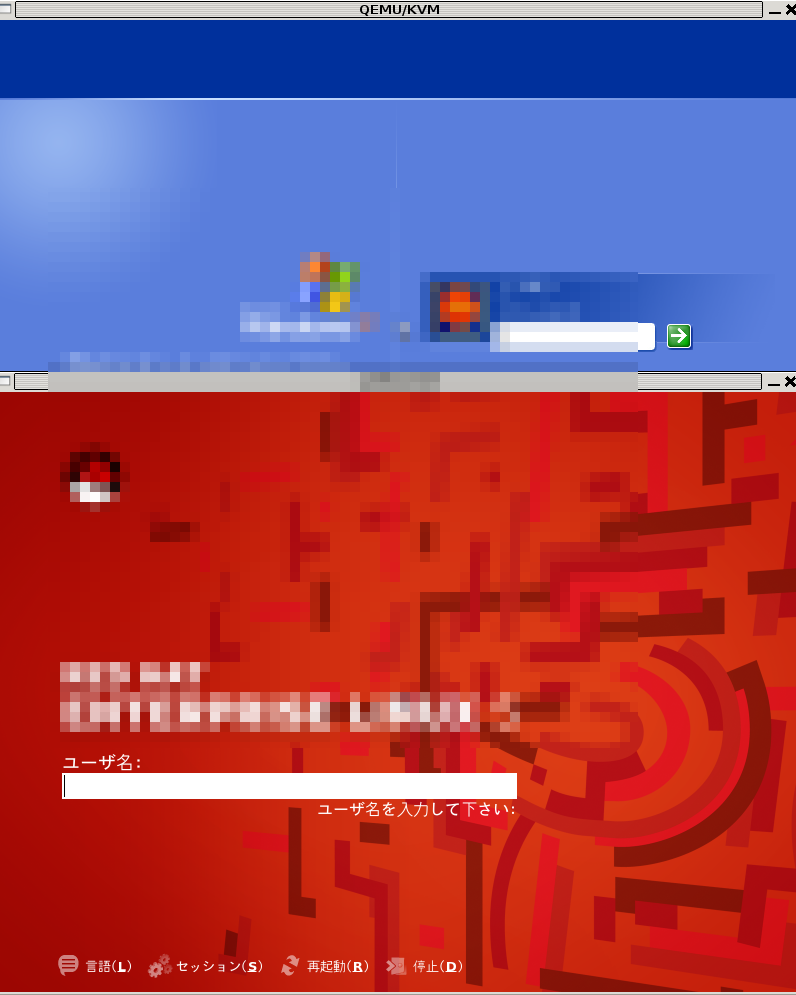
\includegraphics[width=5cm]{image200701/kvm.png}\end{wrapfigure}

Linus Kernel 2.6.20 以降ではカーネル側の機構は標準で入っているようです。
\footnote{2.6.20-rc1 で導入され、まだ 2.6.20 はリリースされていないため
この記事の内容は1月19日時点での予測です} Debian で KVM を利用する際の手
順を説明します。

\texttt{apt-get install kvm} でパッケージをインストールします。kvm コマ
ンドがインストールされます。これが kvm 向けに変更された qemu です。

udev が作成してくれる \texttt{/dev/kvm} にアクセスできるようにします。 
デフォルトは\texttt{ root:kvm 660}\footnote{バージョン11-1以降の場合} で、rootのみがアクセスできる設定になっ
ています。ユーザを kvm グループに追加すればよいでしょう。

\begin{commandline}
# adduser dancer kvm
\end{commandline}

CPUのVT機能はデフォルトで on になっていない場合があるので、 on にします。
これはマシンによって違うようです。 通常 BIOS で設定します。 旧モデルの MacBook の場
合は EFI 上で必要なコマンドを発行することになります。
\footnote{\texttt{vmx-var-set.efi}という名前で流通しているようです。}

以上で、kvm コマンドを利用してVTの恩恵にあずかることができるようになりま
す。コマンドラインなどはqemu 互換、むしろ qemu そのものを利用しているの
で、qemu と同じように動かすことができます。


\subsection{実行例}


kvm を活用していろいろと試してみましょう。qemu 用のディスクイメージを作
成し、適当なディストリビューションのディスクイメージを利用して、インストー
ルします。おそらく、-monitorコマンドで stdio をモニタにするほうが便利で
しょう。

\begin{commandline}
$ qemu-img create -f qcow hda 10G
$ kvm -hda hda -cdrom /home/iso/RHEL4-U4-i386-AS-disc1.iso
   -boot d -m 512 -monitor stdio
(qemu) change cdrom /home/iso/RHEL4-U4-i386-AS-disc2.iso
(qemu) change cdrom /home/iso/RHEL4-U4-i386-AS-disc3.iso
(qemu) change cdrom /home/iso/RHEL4-U4-i386-AS-disc4.iso
(qemu) change cdrom /home/iso/RHEL4-U4-i386-AS-disc5.iso
(qemu) change cdrom /home/iso/RHEL4-U4-i386-AS-disc1.iso
(qemu) eject cdrom
\end{commandline}

ここでは某CDROMが5枚あるディストリビューションを例にとっていますが、
CDROMが5枚あっても、qemu モニターにてCDROMを入れ換えながらGUI操作を行う
ことで無事にインストール完了します。リブートするところでゲストOSがカーネ
ルパニックを起こしますが、そこは適当に kvm 自体を起動しなおせば問題あり
ません。

\begin{commandline}
$ kvm -hda hda  -boot c -m 512 -monitor stdio -localtime  \
 -redir tcp:2222::22
\end{commandline}


\subsection{ベンチマークしてみた}

qemu を使った場合と kvm を使った場合の速度比較をしてみました。まず、ユー
ザ空間で完結する例として単純に while でループを回すだけのプログラムです。
qemu の場合は 6s かかったものが、 kvm の場合は 0.6s で完了しました。

\subsection{パフォーマンスの見えかた}

kvm を実行しているホストOSからどのように見えるのか確認してみましょう。
kvm の仕組だと、システムコールを実行して処理を行うことになるのでしょう。

\texttt{mpstat -P ALL 1} の出力を一部みてみると、一つのCPUの システム時
間がとられているように見えます。

\begin{commandline}
00時28分51秒  CPU   %user   %nice    %sys %iowait    %irq   %soft  %steal   %idle    intr/s
00時28分52秒  all    0.00    0.00   50.00    0.50    0.00    0.50    0.00   49.00   1421.78
00時28分52秒    0    0.00    0.00   92.08    0.00    0.00    0.99    0.00    6.93    430.69
00時28分52秒    1    0.00    0.00    6.93    0.99    0.00    0.00    0.00   91.09    991.09
\end{commandline}

\texttt{top}コマンドで見た場合には、kvmは通常のプロセスと同様にCPU時間を
消費し、メモリを消費しているように見えます。

\begin{commandline}
  PID USER      PR  NI  VIRT  RES  SHR S %CPU %MEM    TIME+  COMMAND
 3746 dancer    25   0  308m 252m 246m R   82 25.7 100:36.60 kvm
 2512 root      10  -5     0    0    0 S    0  0.0   0:11.32 kjournald
 2806 root      15   0  2556  932  804 S    0  0.1   1:09.36 syslogd
\end{commandline}

\texttt{iostat 1 /dev/dm-1 }の出力を確認してみます。
ゲストOSのディスクIOによってホストOSのディスクIOが発生しているのが見れます。

\begin{commandline}
avg-cpu:  %user   %nice %system %iowait  %steal   %idle
           0.00    0.00   42.50   42.00    0.00   15.50

Device:            tps   Blk_read/s   Blk_wrtn/s   Blk_read   Blk_wrtn
dm-1            805.94       102.97      6400.00        104       6464
\end{commandline}

\subsection{他との比較}

Xen, qemu, qemu+kqemu, openvz, vserver, user-mode-linux などと機能を比較
してみましょう。と思ったらすでにやられていたので、このURLを参照してくだ
さい。\url{http://virt.kernelnewbies.org/TechComparison}

\cleartoevenpage

\begin{minipage}[b]{0.2\hsize}
 \definecolor{titleback}{gray}{0.9}
 \colorbox{titleback}{\rotatebox{90}{\fontsize{80}{80} {\gt デビアン勉強会} }}
\end{minipage}
\begin{minipage}[b]{0.8\hsize}

\vspace*{15cm}
\hrule
\vspace{2mm}

\includegraphics[width=2cm]{image200502/openlogo-nd.eps}
\noindent \Large \bf Debian 勉強会資料\\ \\
\noindent \normalfont \debmtgyear{}年\debmtgmonth{}月\debmtgdate{}日 \hspace{5mm}  初版第1刷発行\\
\noindent \normalfont 東京エリア Debian 勉強会 (編集・印刷・発行)\\
\hrule
\end{minipage}

\end{document}
